\chapter{Figures}


\begin{figure}[h]
    \begin{minipage}[c]{0.5\linewidth}
        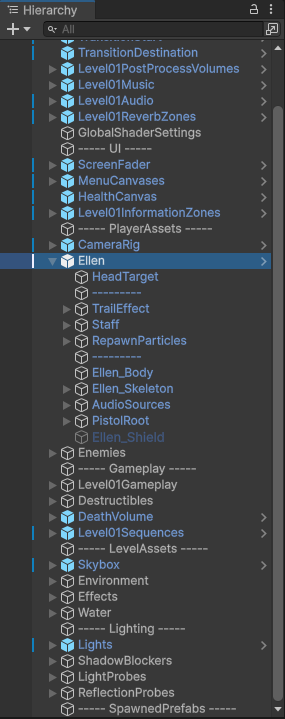
\includegraphics[width=0.9\textwidth]{content/Research/Unity-Hierarchy.png}
        \caption{Screenshot of the Unity engine's Hierarchy view, showing a tree of all the Game Objects present in the scene.}
        \label{fig:unity-hierarchy}
    \end{minipage}
    \hfill
    \begin{minipage}[c]{0.5\linewidth}
        \includegraphics[width=\textwidth]{content/Research/Unity-Inspector.png}
        \caption{Screenshot of the Unity engine's Inspector view, showing the properties and components of a selected Game Object.}
        \label{fig:unity-inspector}
    \end{minipage}%
\end{figure}


\begin{figure}[h]
    \begin{minipage}[c]{0.5\linewidth}
        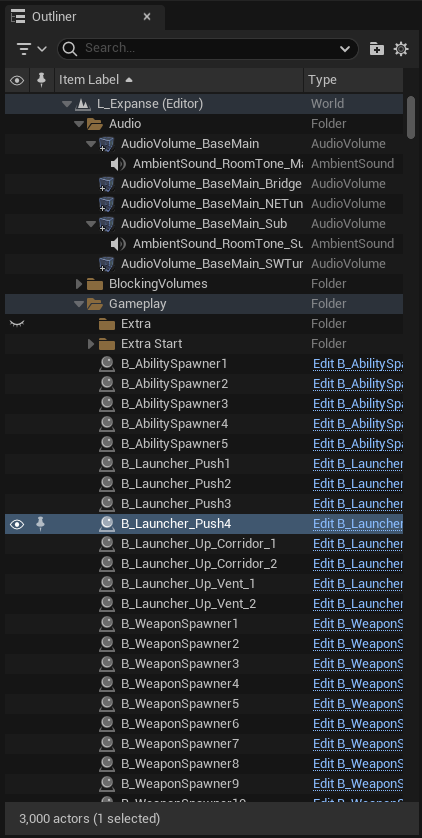
\includegraphics[width=0.9\textwidth]{content/Research/UE5-Outliner}
        \caption{Screenshot of the Unreal Engine's Outliner view, showing a tree of all the Actors present in the scene}
        \label{fig:ue5-outliner}
    \end{minipage}
    \hfill
    \begin{minipage}[c]{0.5\linewidth}
        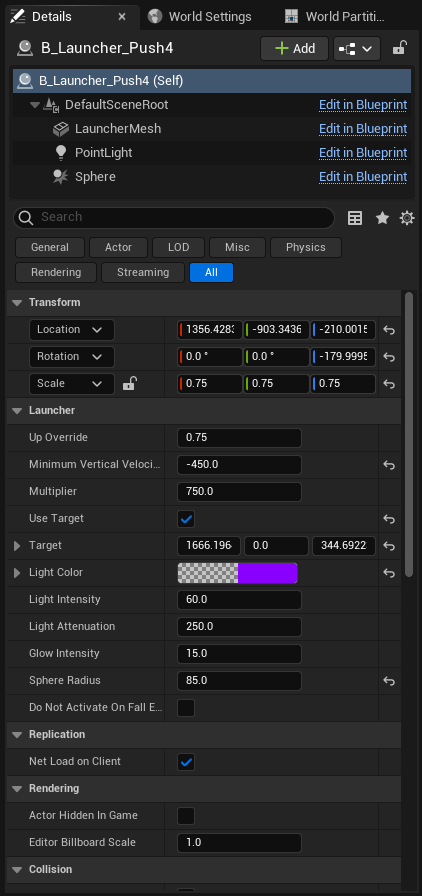
\includegraphics[width=\textwidth]{content/Research/UE5-Details}
        \caption{Screenshot of the Unreal Engine's Details view, showing the properties and components of a selected Actor.}
        \label{fig:ue5-details}
    \end{minipage}%
\end{figure}


\begin{figure}
    \includegraphics[width=1\textwidth]{content/architecture/startup.eps}
    \caption{Sequence diagram of the start-up of the engine}
    \label{fig:startup-diagram}
\end{figure}

\begin{figure}
    \includegraphics[width=1\textwidth]{content/architecture/startup-init.eps}
    \caption{Detailed sequence diagram of module initialization}
    \label{fig:startup-init-diagram}
\end{figure}